\chapter{Kubernetes}
Als Resultat jahrelanger Erfahrung die Google im Bau von Container-Anwendungen, sowie deren Betrieb in Clustern gemacht hat, bildet Kubernetes eines der wohl am häufigsten genutzten Managementtools für Container innerhalb eines Docker Clusters.\\
Von Beginn an dazu entwickelt Deployment und Skalierung von Containern zu automatisieren, hat sich das am 07. Juni 2014 als Open Source Plattform erstmals vorgestellte Kubernetes neben Apaches Mesos oder Hadoop YARN etabliert und wird im folgenden Kapitel vorgestellt.\\
Dabei werden verschiedene Aspekte wie Architektur, Skalierung oder Persistenz betrachtet und ein Vergleich zu Docker Swarm als Alternative gezogen.


\section{Architektur}
\begin{figure}
	\centering
	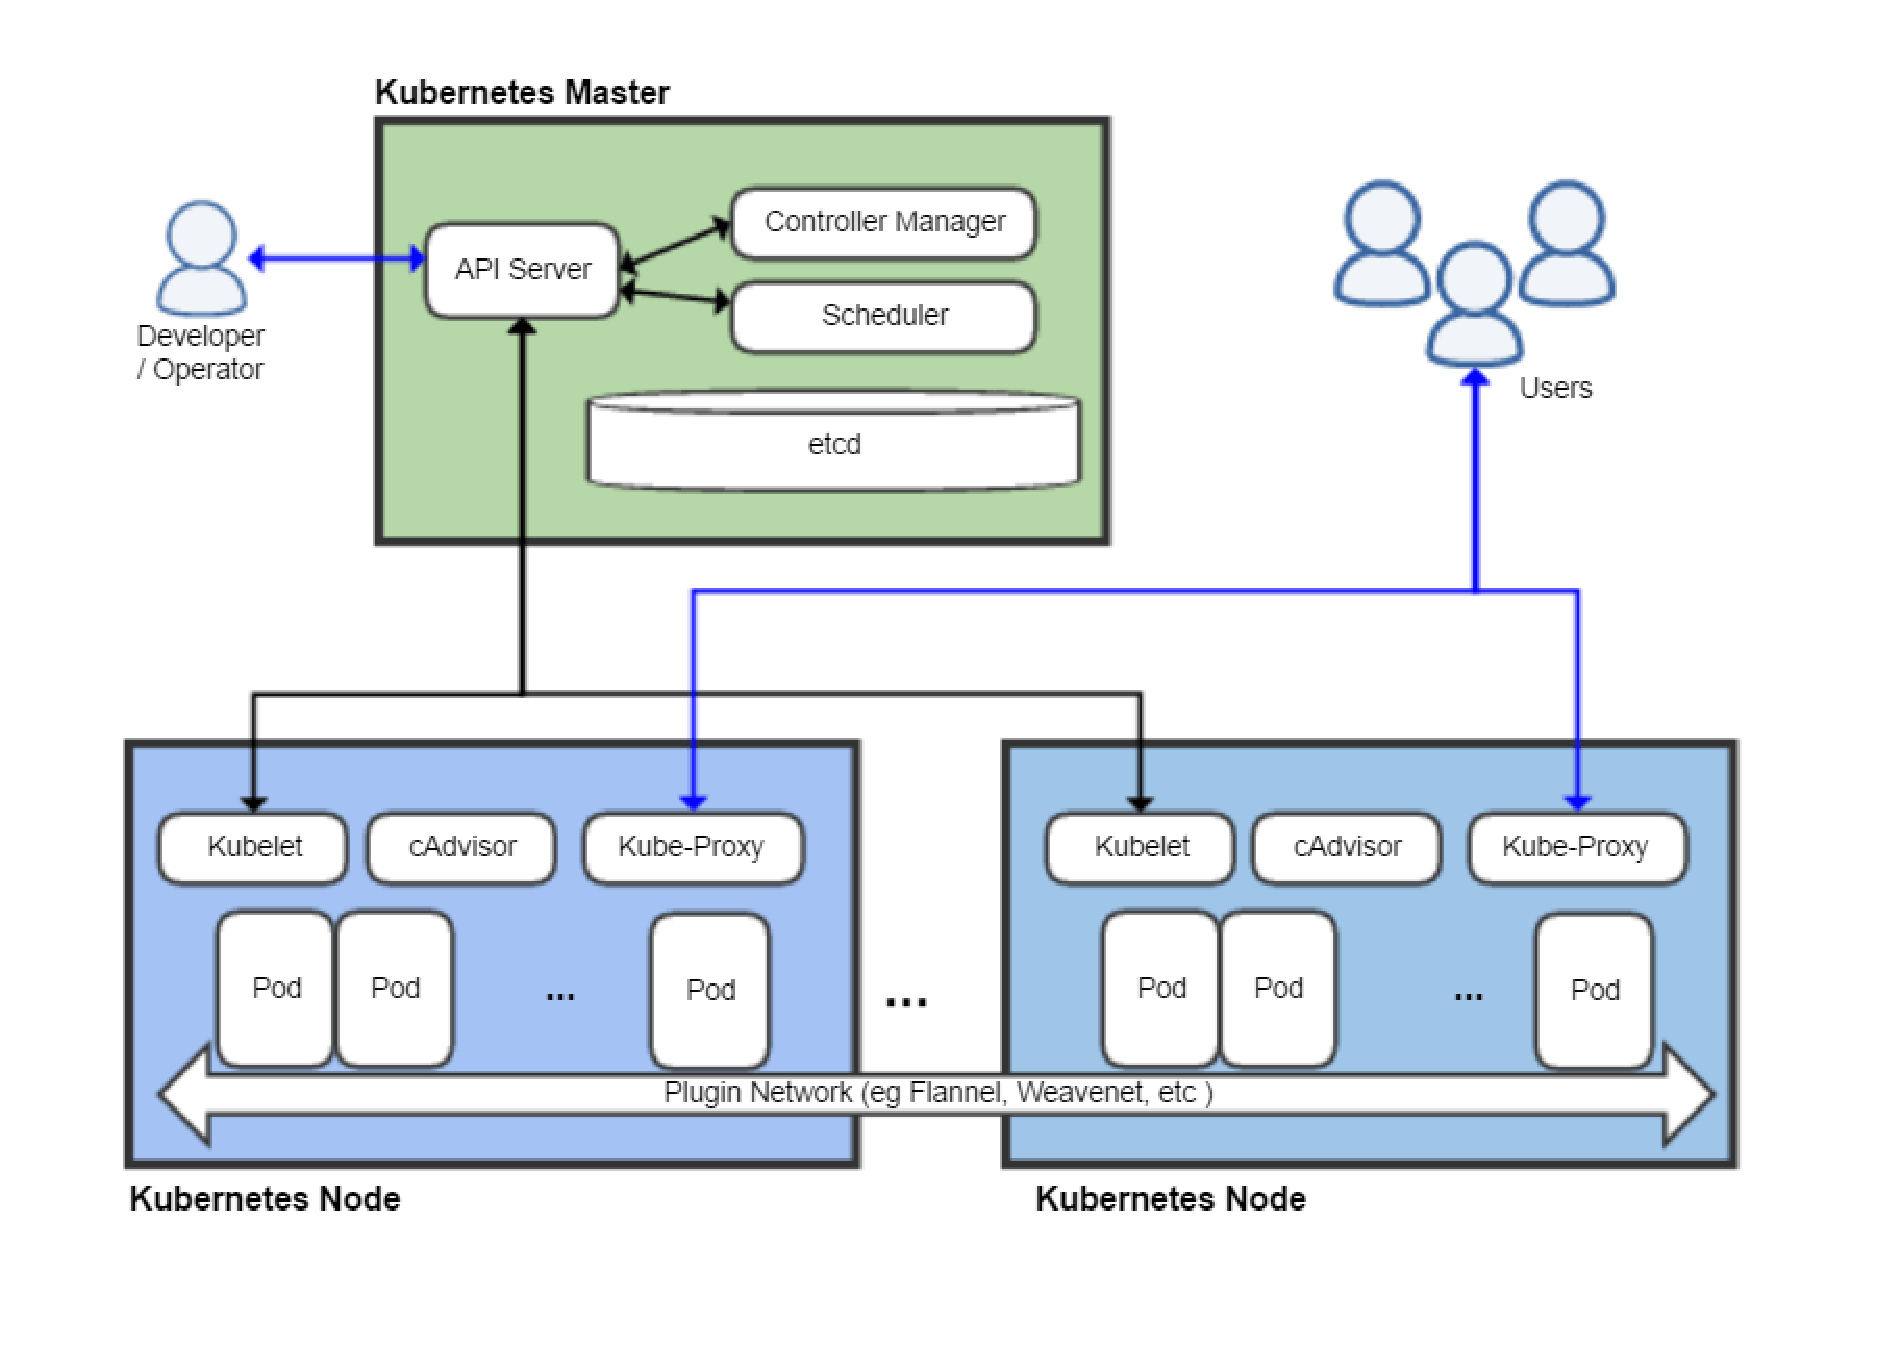
\includegraphics[width=0.9\linewidth]{figures/kubernetes-architecture}
	\caption[Kubernetes Architekture]{Kubernetes Architektur im Cluster}
	\label{fig:kubernetes-architecture}
\end{figure}
Die Architektur von Kubernetes entspricht dem Master-Slave Prinzip wie Abbildung \ref{fig:kubernetes-architecture} schematisch zeigt. Dabei steuert der Master die Nodes auf denen die Docker Container laufen.\\
Der Kubernetes Master ist besteht im wesentlichen aus drei Prozessen die auf einem einzelnen Knoten des Clusters laufen. Dieser wird häufig auch Master Node genannt und besteht aus folgenden Komponenten:
\begin{itemize}
	\item API Server - zentrale Komponente, die via REST Schnittstelle allen anderen Komponenten Informationen bereitstellt.
	\item Scheduler - überwacht die Last der einzelnen Nodes und entscheidet abhängig von verfügbaren Ressourcen auf welcher Node weitere Pods gestartet werden.
	\item Controller Manager - enthält alle Kontrollmechanismen und kommuniziert mit dem API Server um den aktuellen Zustands des Clusters zu überwachen und diesen in den gewünschten Zustand zu überführen.
	\item etcd - leichtgewichtige Key-Value Datenbank zur Speicherung der Cluster Konfiguration. Diese Enthält den Gesamtzustand des Clusters und wird vom API Server genutzt.
\end{itemize}\newpage
Die übrigen Nodes, ehemals Minions genannt, bilden einzelne Server auf denen Container gestartet werden können. Jeder Node stellt eine Container Laufzeitumgebung zur Verfügung und besteht aus folgenden Komponenten:
\begin{itemize}
	\item Kubelet - zentrale Komponente einer Node und überwacht als solche den aktuellen Status der Node und meldet diese an den Controller Manager. Dieser gibt dann Anweisung zum Starten oder Stoppen von Containern. Fällt ein Container aus wird er vom Kubelet auf der gleichen Node neu gestartet. Fällt die komplette Node aus, wird dies vom Master aufgrund ausbleibender Statusmeldung erkannt und die Pods werden auf anderen Nodes neu gestartet.
	\item Kube-Proxy - implementiert Netzwerk Proxy und Load Balancer. Routet abhängig von IP Adresse und Port eingehenden Netzwerkverkehr an die entsprechenden Container.
	\item cAdvisor - ist im Kubelet integriert und zeichnet die Resourcen eines Containers auf, um diese anderen Monitoringlösungen zur Auswertung von Metriken bereitzustellen.
\end{itemize}
\section{Skalierung}

\section{Persistenz}

\section{Service Discovery und Load Balancing}

\section{Batch Exectution}